% Author: Andreas Hermann
% this can just simply be included into a main documenty via
% \includegraphics[width=1\textwidth]{04_images/sota_taxonomy}

\documentclass[tikz]{standalone}

\usepackage{tikz}
\usepackage[utf8]{inputenc}
\usetikzlibrary{mindmap,trees}
\begin{document}
\pagestyle{empty}

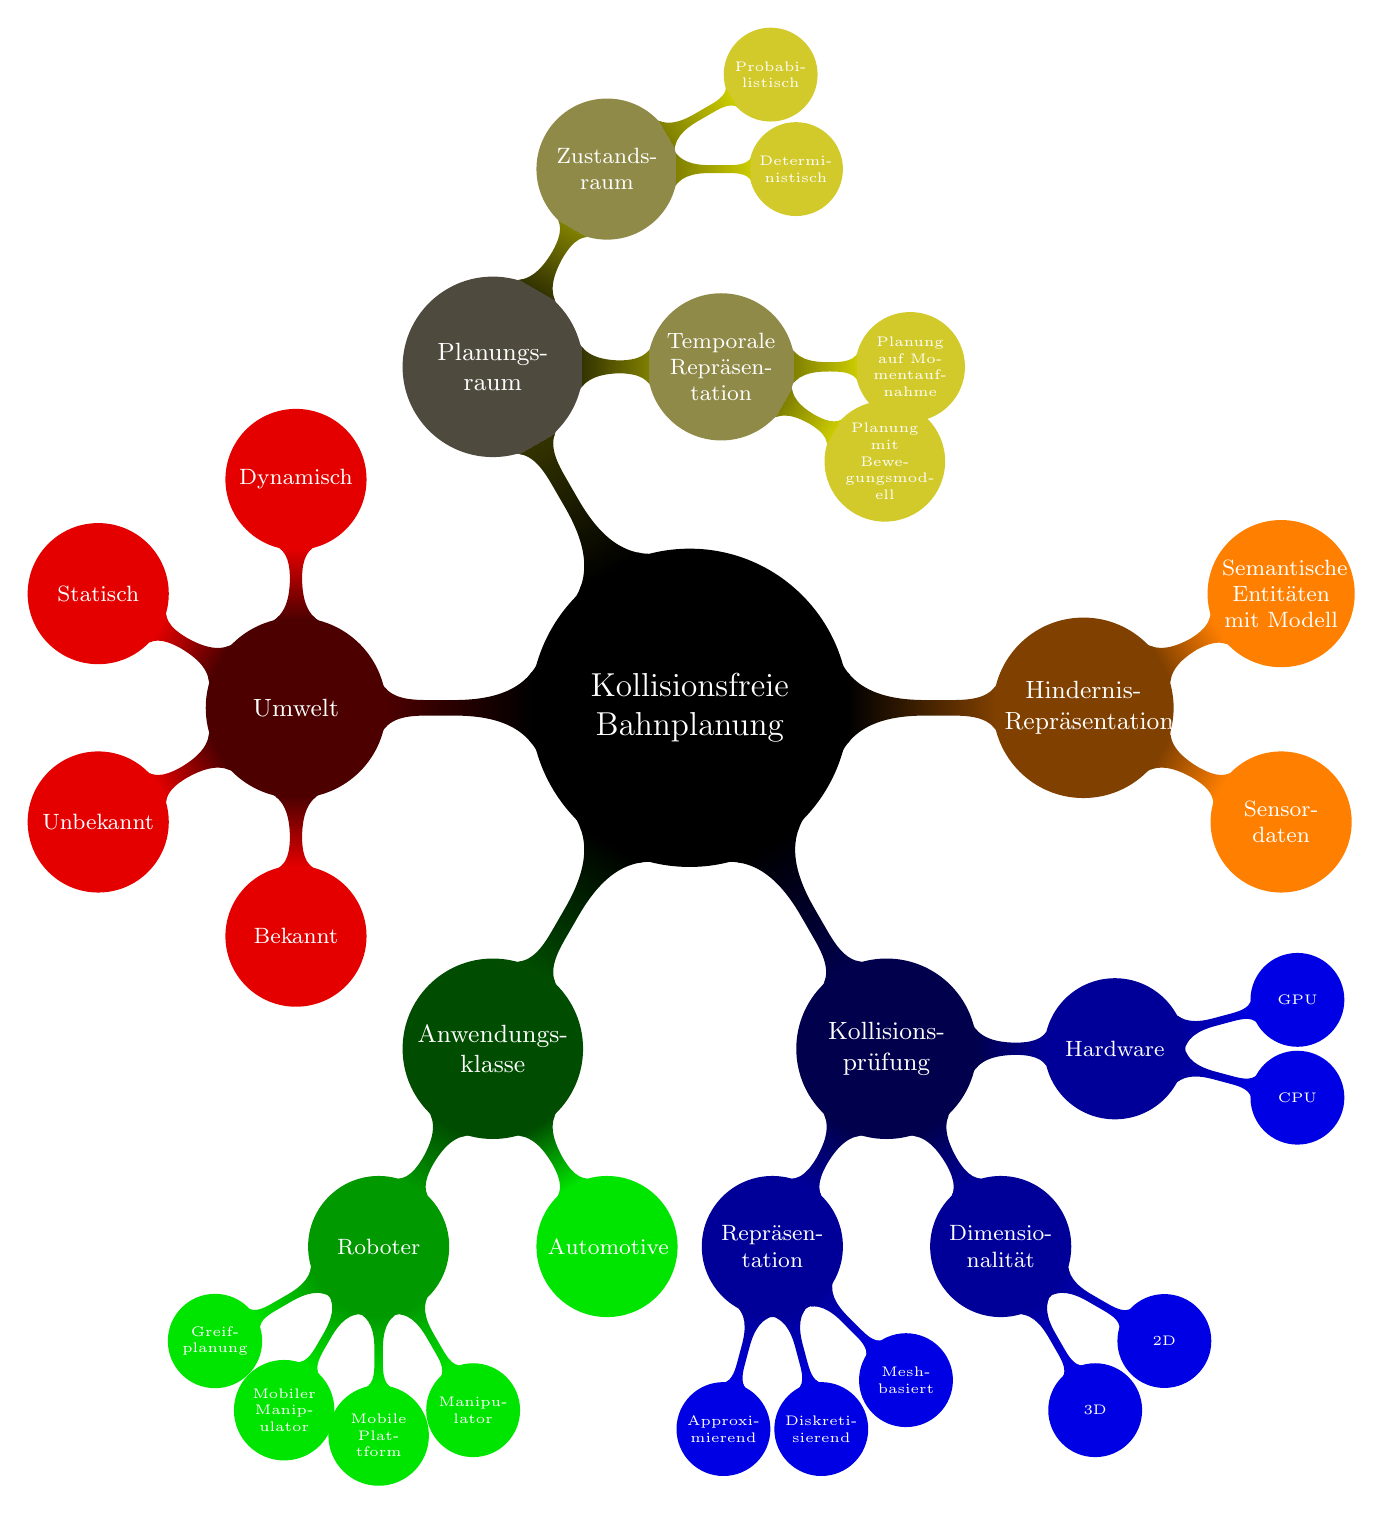
\begin{tikzpicture}
  \path[mindmap,concept color=black,text=white]
  
	node[concept] {Kollisionsfreie Bahnplanung}
	[clockwise from=0]
    child[concept color=orange!50!black] { 
		node[concept] {Hindernis-Repräsentation} 
    		[clockwise from=30]    
		child[concept color=orange] { node[concept] {Semantische Entitäten mit Modell} }
		child[concept color=orange] { node[concept] {Sensor-daten} }
	}
	child[concept color=blue!30!black] {
		node[concept] {Kollisions-prüfung}
		[clockwise from=0]
		child[concept color=blue!60!black] {
    			node[concept] {Hardware}
            [clockwise from=15]
            child[concept color=blue!90!black] { node[concept] {GPU} }
            child[concept color=blue!90!black] { node[concept] {CPU} }
		}
        child[concept color=blue!60!black] { 
			node[concept] {Dimensio-nalität}
			[clockwise from=-30]    
			child[concept color=blue!90!black] { node[concept] {2D} }
			child[concept color=blue!90!black] { node[concept] {3D} }
         }
		child[concept color=blue!60!black] {
			node[concept] {Repräsen-tation}
			[clockwise from=-45]
			child[concept color=blue!90!black] { node[concept] {Mesh-basiert} }
			child[concept color=blue!90!black] { node[concept] {Diskreti-sierend} }
			child[concept color=blue!90!black] { node[concept] {Approxi-mierend} }
    		}
    }  
    child[concept color=green!30!black] {
		node[concept] {Anwendungs-klasse}
		[clockwise from=-60]
		child[concept color=green!90!black] { node[concept] {Automotive} }
		child[concept color=green!60!black] { 
			node[concept] {Roboter} 
			[clockwise from=-60]    
			child[concept color=green!90!black] { node[concept] {Manipu-lator} }
			child[concept color=green!90!black] { node[concept] {Mobile Plattform} }
			child[concept color=green!90!black] { node[concept] {Mobiler Manipulator} }
			child[concept color=green!90!black] { node[concept] {Greif-planung} }
         }
    }
    child[concept color=red!30!black] { 
		node[concept] {Umwelt}
		[clockwise from=-90]
		child[concept color=red!90!black] { node[concept] {Bekannt} }
		child[concept color=red!90!black] { node[concept] {Unbekannt} }
		child[concept color=red!90!black] { node[concept] {Statisch} }
		child[concept color=red!90!black] { node[concept] {Dynamisch} }      
	}
	child[concept color=yellow!20!black] { 
		node[concept] {Planungs-raum}
		[clockwise from=60]
		child[concept color=yellow!50!black] { 
			node[concept] {Zustands-raum} 
			[clockwise from=30]
			child[concept color=yellow!80!black] { node[concept] {Probabi-listisch} }
			child[concept color=yellow!80!black] { node[concept] {Determi-nistisch} }
		}
		child[concept color=yellow!50!black] { 
			node[concept] {Temporale Repräsen-tation} 
			[clockwise from=0]
			child[concept color=yellow!80!black] { node[concept] {Planung auf Momentaufnahme} }
			child[concept color=yellow!80!black] { node[concept] {Planung mit Bewegungsmodell} }
		}
	};
\end{tikzpicture}
\end{document}
